% Copyright 2004 by Till Tantau <tantau@users.sourceforge.net>.
%
% In principle, this file can be redistributed and/or modified under
% the terms of the GNU Public License, version 2.
%
% However, this file is supposed to be a template to be modified
% for your own needs. For this reason, if you use this file as a
% template and not specifically distribute it as part of a another
% package/program, I grant the extra permission to freely copy and
% modify this file as you see fit and even to delete this copyright
% notice.

\documentclass{beamer}

%\usetheme{Madrid}
%\usecolortheme{beaver}

%\usetheme{Berlin}

\usetheme{CambridgeUS}
%\usecolortheme{default}

\usecolortheme{beaver}

\usefonttheme{professionalfonts} % using non standard fonts for beamer
\usefonttheme{serif} % default family is serif
\usepackage{fontspec} % Allows font customization
\defaultfontfeatures{Mapping=tex-text,Scale=MatchLowercase}
\setmainfont{Ubuntu Light} % Main document font

\usepackage{hyperref}
\usepackage[english,spanish]{babel}
\usepackage{multicol} % Split TOC into two colums

\title{Fusión de imágenes con Poisson}

% A subtitle is optional and this may be deleted
\subtitle{Universidad de Granada}

\author{Cristina~Heredia, Alejandro~Alcalde}
% - Give the names in the same order as the appear in the paper.
% - Use the \inst{?} command only if the authors have different
%   affiliation.

\institute[ETSIIT] % (optional, but mostly needed)
{}
% - Use the \inst command only if there are several affiliations.
% - Keep it simple, no one is interested in your street address.

\date{\today}
% - Either use conference name or its abbreviation.
% - Not really informative to the audience, more for people (including
%   yourself) who are reading the slides online

\subject{Fusión de imágenes con Poisson}
% This is only inserted into the PDF information catalog. Can be left
% out.

% If you have a file called "university-logo-filename.xxx", where xxx
% is a graphic format that can be processed by latex or pdflatex,
% resp., then you can add a logo as follows:

%\pgfdeclareimage[height=0.1cm]{university-logo}{university-logo-filename}
%\logo{\pgfuseimage{university-logo}}
%\titlegraphic{\includegraphics{university-logo-filename}}

% Delete this, if you do not want the table of contents to pop up at
% the beginning of each subsection:
\AtBeginSubsection[]
{
  \begin{frame}<beamer>[allowframebreaks]{Contenidos}
  \begin{multicols}{2}
    \tableofcontents[currentsection,currentsubsection]
  \end{multicols}
  \end{frame}
}

\AtBeginSection[]
{
  \begin{frame}<beamer>[allowframebreaks]{Contenidos}
  \begin{multicols}{2}
    \tableofcontents[currentsection,currentsubsection]
  \end{multicols}
  \end{frame}
}

% Let's get started
\begin{document}

\begin{frame}
  \titlepage
\end{frame}

\begin{frame}{Contenidos}
\begin{multicols}{2}
  \tableofcontents
  % You might wish to add the option [pausesections]
\end{multicols}
\end{frame}

\section{Problema}

% You can reveal the parts of a slide one at a time
% with the \pause command:
\begin{frame}{Problema}
  \begin{itemize}
    \item Edición de imágenes a nivel local. Aplicar cambios a una región de una imagen.
    \item<2-> Planteamiento: 3 Ecuaciones de Poisson usando Cholesky.
    \item<3-> Espacio de trabajo: \textit{RGB}.
  \end{itemize}
\end{frame}

\section{Procedimiento y solución de Poisson}
\begin{frame}{Procedimiento y solución de Poisson}
  \begin{itemize}
    \item Minimizar: \[min_{f}\int \int_{\Omega} \parallel \bigtriangledown f-V\parallel^{2}\] con \[f|\partial_{\Omega}=f^{*}|\partial_{\Omega}\] V es el guidance field.
    \item<2-> \[\bigtriangledown =\left [\frac{\partial }{\partial x},\frac{\partial }{\partial y} \right ]\] Operador de gradiente
    \item<3->
  \end{itemize}
\end{frame}

\begin{frame}{Procedimiento y solución de Poisson}
  \begin{itemize}
    \item Su solución es la única solución a la ecuación: $\Delta f=div V$ con $f|\partial_{\Omega}=f^{*}|\partial_{\Omega}$
    \item<2-> $\Delta=\frac{\partial^2 }{\partial x^2}+\frac{\partial^2 }{\partial y^2}$ es el operador
    Laplaciano.
    \item<3-> $div=\frac{\partial }{\partial x}+\frac{\partial }{\partial y}$ es el operador de divergencia.
    \item<4-> Para nosotros: Resolver 3 ec $Ax=b$, de donde $x=A ^{-1}*b$ o $x=A\setminus b$
    \item<5-> $A$ es la matriz de coeficientes ($NxN$ pixeles a copiar), $b$ el vector solución (\textit{Guidance field})
  \end{itemize}
\end{frame}

\begin{frame}{Procedimiento y solución de Poisson}
  \begin{block}{}
  La matriz $A$ es de la forma
  \begin{figure}[H]
  \centering
  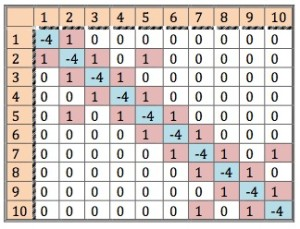
\includegraphics[scale=.4]{./img/kernel}
  \end{figure}
  $b$ es un vector de tres filas (Una por cada canal) y $n$ columnas (Los píxeles de la máscara).
  \end{block}
\end{frame}

\begin{frame}{Procedimiento y solución de Poisson}
  \begin{itemize}
    \item \[ v =\sum_{q\epsilon N_{p}\bigcap \partial\Omega}f^{*}_{q}+\sum_{q\epsilon N_{p}}v_{pq}\]
    \item<2-> El primer termino es la suma de los píxeles vecinos de $p$ que pertenecen a la parte negra de la máscara (No seleccionados), y por tanto son parte de la imagen destino.
    \item<3-> El segundo termino es el gradiente de la imagen. (Se calcula distinto en \textit{normal seamless cloning} y \textit{mixin seamless clonning}  )
  \end{itemize}
\end{frame}

\begin{frame}{Normal Seamless cloning}
  \begin{itemize}
    \item EL gradiente en este caso se obtiene como $v= \bigtriangledown g $, donde $g$ es la imagen fuente.
    \item<2-> Discretizado se traduce en $\forall <p,q>,v_{pq} =g_{p}-g_{q}$. En general buenos resultados si la imagen no presenta transparencias.
  \end{itemize}
\end{frame}

\begin{frame}{Mixin Seamless cloning}
  \begin{itemize}
    \item Mejora el seamless cloning cuando la imagen fuente tiene transparencias.
    \item<2-> Se calcula el guidance Vect tomando el gradiente más fuerte entre la imágen fuente y la imágen de destino.
    \item<3-> $v_{pq}=\left\{\begin{matrix} f^{*}_{p}-f^{*}_{q}$ if $\mid f^{*}_{p}-f^{*}_{q}\mid > \mid g_{p}-g_{q} \mid \\ g_{p}-g_{q} \end{matrix}\right.$
  \end{itemize}
\end{frame}

\begin{frame}{Ejemplos Mixin Seamless}
  \begin{block}{}
  \begin{figure}[H]
  \centering
  
\includegraphics[scale=1]{./img/nube_src}
  \end{figure}
  \end{block}
\end{frame}

\begin{frame}{Ejemplos Mixin Seamless}
  \begin{block}{}
  \begin{figure}[H]
  \centering
  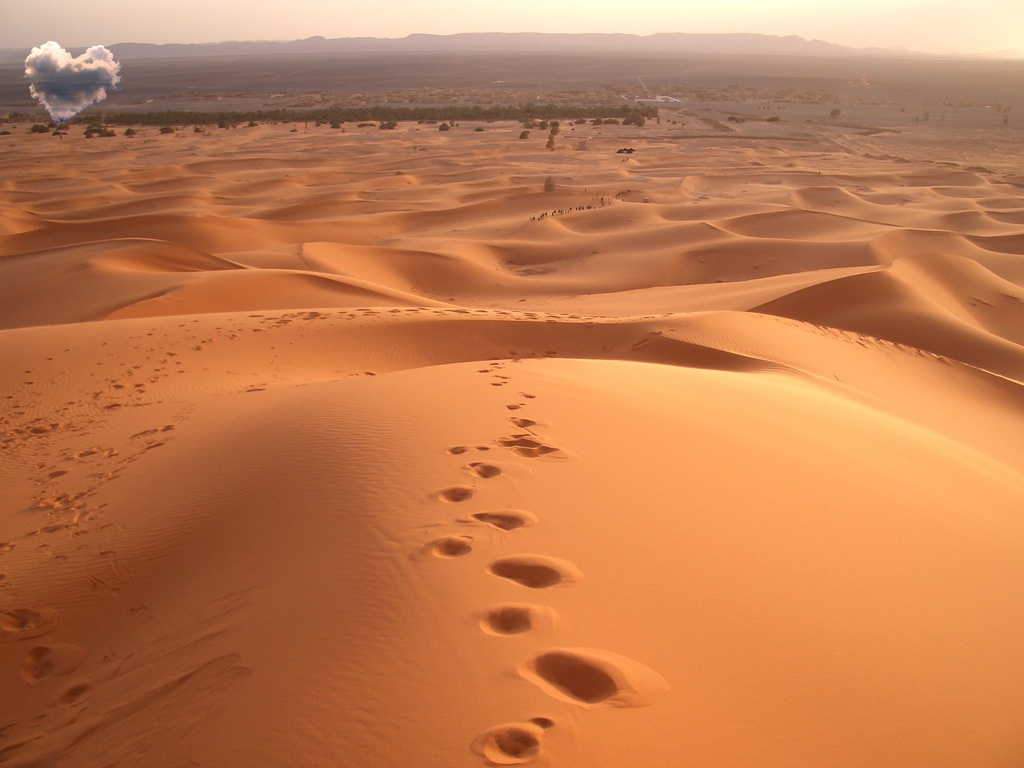
\includegraphics[scale=.5]{./img/desertnube}
  \end{figure}
  \end{block}
\end{frame}

\begin{frame}{Ejemplos Normal Seamless}
  \begin{block}{}
  \begin{figure}[H]
  \centering
  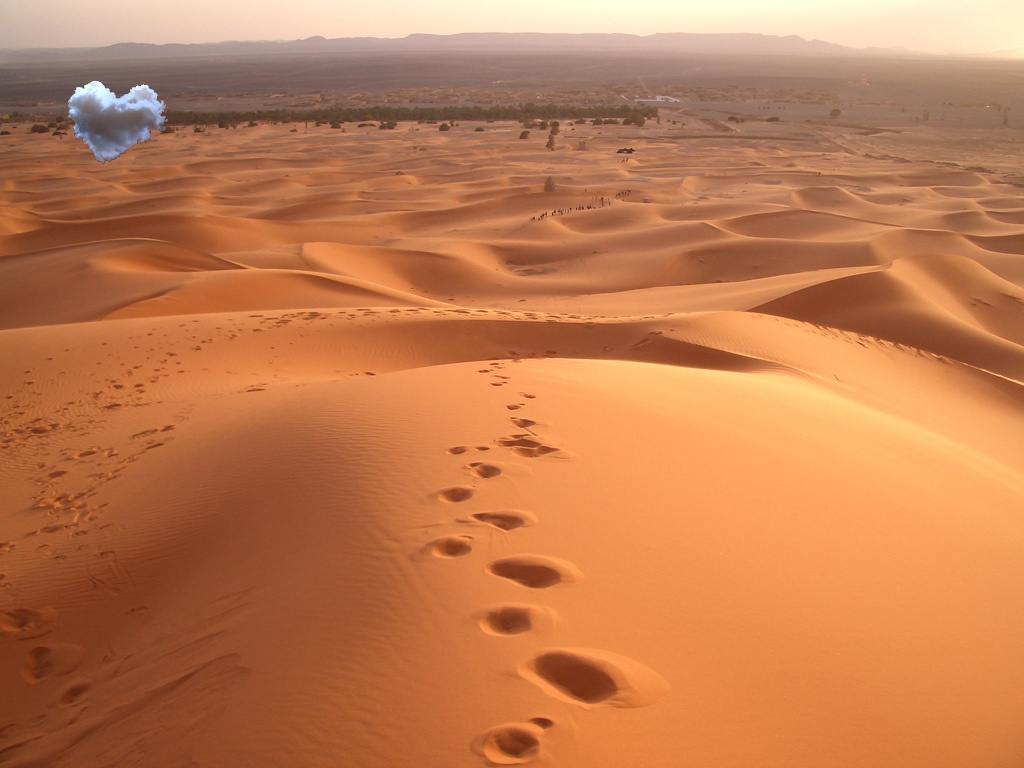
\includegraphics[scale=.5]{./img/normalblue}
  \end{figure}
  \end{block}
\end{frame}

\begin{frame}{Ejemplos mixin Seamless}
  \begin{block}{}
  \begin{figure}[H]
  \centering
  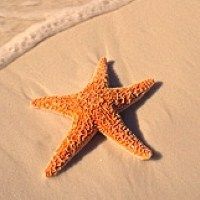
\includegraphics[scale=.5]{./img/estrella_src.jpg}
  \end{figure}
  \end{block}
\end{frame}

\begin{frame}{Ejemplos mixin Seamless}
  \begin{block}{}
  \begin{figure}[H]
  \centering
  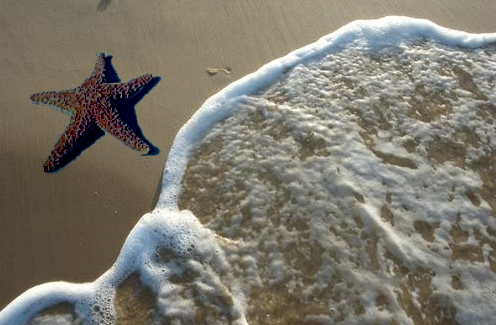
\includegraphics[scale=.5]{./img/mix_seastar}
  \end{figure}
  \end{block}
\end{frame}


% All of the following is optional and typically not needed.
\appendix
\section<presentation>*{\appendixname}
\subsection<presentation>*{Bibliografía recomendada}

\begin{frame}[allowframebreaks]
  \frametitle<presentation>{Bibliografía}

  \bibliography{biblio}{}
  \bibliographystyle{IEEEtran}

  \nocite{*}

\end{frame}

\end{document}
